\subsection{Kế hoạch và phân công công việc giai đoạn 1}

\renewcommand{\arraystretch}{1.3}

\begin{longtable}{|>{\centering\arraybackslash}m{1.5cm}|m{7cm}|m{5cm}|}
	\hline
	\textbf{Tuần} & \textbf{Công việc} & \textbf{Người thực hiện} \\
	\hline
	\endfirsthead
	
	\hline
	\textbf{Tuần} & \textbf{Công việc} & \textbf{Người thực hiện} \\
	\hline
	\endhead
	
	\hline
	\endfoot
	
	38-39 & Xác định phạm vi đề tài: xây dựng website học toán tư duy cho học sinh tiểu học & Nguyễn Văn Thành \\
	\cline{2-3}
	& Xác định đối tượng người dùng, stakeholders và hệ thống liên quan & Trương Anh Khoa \\
	\cline{2-3}
	& Thống nhất yêu cầu người dùng và các chức năng cần thiết & Nguyễn Văn Thành, \newline Nguyễn Minh Tân, \newline Trương Anh Khoa \\
	\cline{2-3}
	& Thiết kế giao diện người dùng: Trang Landing, Trang chủ (học sinh), Trang Bài học và giao diện popup quản lý tài khoản người dùng. & Nguyễn Minh Tân \\
	\hline
	
	40-41 & Vẽ usecase diagram cho toàn bộ hệ thống và activity diagram cho các luồng Đăng nhập, Đăng ký, Làm bài tập. & Trương Anh Khoa \\
	\cline{2-3}
	& Vẽ sequence diagram cho các luồng Đăng nhập, Đăng ký, Làm bài tập. & Nguyễn Minh Tân \\
	\cline{2-3}
	& Thiết kế cơ sở dữ liệu. & Nguyễn Văn Thành \\
	\cline{2-3}
	& Thiết kế giao diện người dùng: Trang Milestone, Trang Đấu trường, Bảng xếp hạng, Trang Nhiệm vụ, Trang Làm bài kiểm tra. & Nguyễn Minh Tân \\
	\hline
	
	42-43 & Thiết kế kiến trúc hệ thống (Frontend – Backend – Database) & Nguyễn Văn Thành \\
	\cline{2-3}
	& Tạo các repository để quản lý mã nguồn cho frontend và backend & Nguyễn Văn Thành, \newline Nguyễn Minh Tân, \newline Trương Anh Khoa \\
	\cline{2-3}
	& Thiết kế giao diện người dùng: Trang Minigame, Trang Thống kê (phụ huynh), Trang Lịch sử làm bài & Nguyễn Minh Tân \\
	\hline
	
	44-45 & Setup backend, cấu hình server, tạo database và các bảng chính & Nguyễn Văn Thành \\
	\cline{2-3}
	& Hiện thực giao diện người dùng: Trang Landing, Trang chủ (học sinh), Trang Đấu trường, Trang Đăng nhập/Đăng ký, Trang Onboarding, Trang Milestone, Trang Lấy lại mật khẩu. & Nguyễn Minh Tân \\
	\cline{2-3}
	& Hiện thực giao diện người dùng: Trang Bài học, Trang Nhiệm vụ, Trang Bảng xếp hạng, giao diện quản lý tài khoản người dùng bao gồm Chỉnh sửa thông tin cá nhân, Đổi mật khẩu, Liên kết tài khoản. & Trương Anh Khoa \\
	\cline{2-3}
	& Hiện thực các API đăng nhập, đăng ký, lấy danh sách các chủ đề theo lớp. & Nguyễn Văn Thành \\
	\hline
	
	46-47 & Thiết kế các dạng bài tập tương tác (nối, đúng/sai, tô màu, kéo thả, điền khuyết) & Trương Anh Khoa \\
	\cline{2-3}
	& Hiện thực các dạng bài tập tương tác. & Trương Anh Khoa \\
	\cline{2-3}
	& Hoàn thiện và nối API cho chức năng đăng nhập và đăng ký tài khoản. & Nguyễn Minh Tân \\
	\cline{2-3}
	& Hiện thực các API quản lý khối lớp, chủ đề, bài tập, cập nhật điểm, quản lý tiến trình học tập & Nguyễn Văn Thành \\
	\hline
	
	48-49 & Hoàn thiện luồng làm bài tập tương tác ở frontend. & Nguyễn Minh Tân, \newline Trương Anh Khoa \\
	\cline{2-3}
	& Thiết kế và hoàn thiện minigame Math Match. & Trương Anh Khoa \\
	\cline{2-3}
	& Hiện thực các API quản lý tài khoản người dùng, gợi ý chủ đề học tập theo thời gian, quản lý đấu trường & Nguyễn Văn Thành \\
	\hline
	
	50-51 & Tối ưu backend, fix bugs, refactor code & Nguyễn Văn Thành \\
	\cline{2-3}
	& Hoàn thiện và nối API cho các chức năng quản lý tài khoản người dùng & Trương Anh Khoa \\
	\cline{2-3}
	& Hoàn thiện và nối API cho các chức năng chơi minigame, hiển thị tiến trình học tập & Nguyễn Minh Tân \\
	\cline{2-3}
	& Kiểm tra lại các chức năng cơ bản đã được hiện thực & Nguyễn Văn Thành, \newline Nguyễn Minh Tân, \newline Trương Anh Khoa \\
	\hline
	
\end{longtable}

\begin{figure}[H]
	\centering
	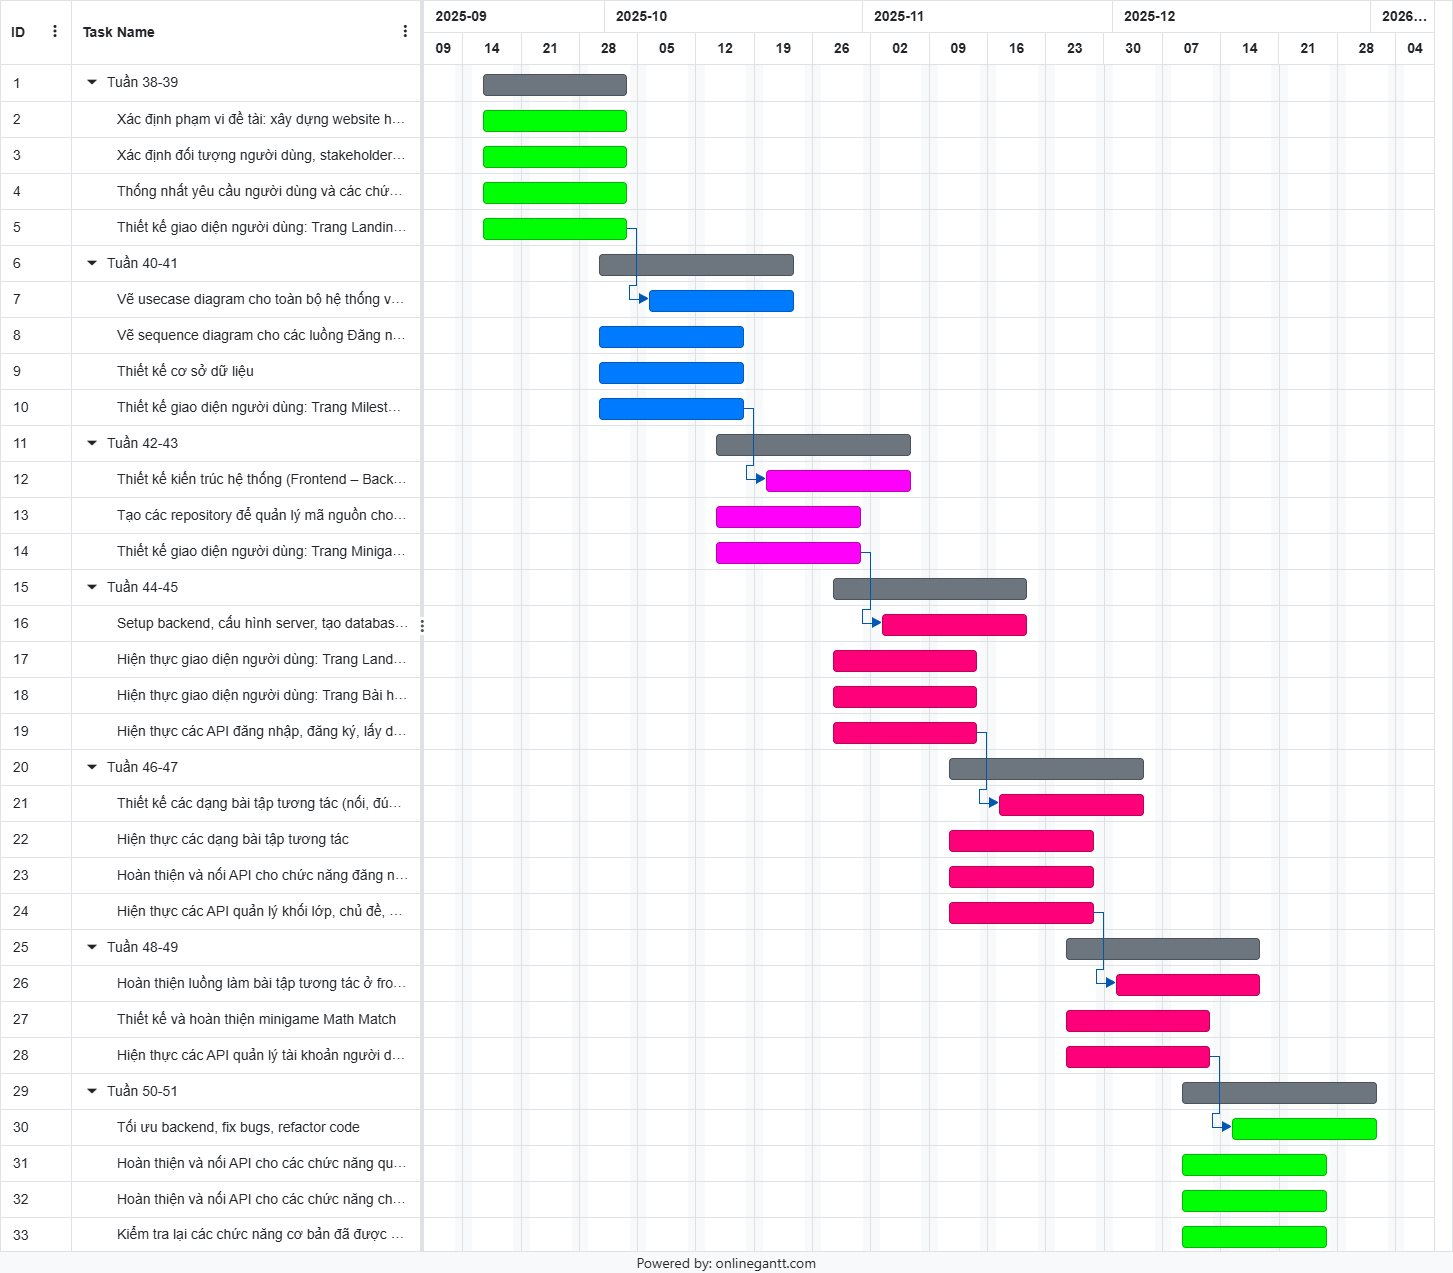
\includegraphics[width=\textwidth]{Image/phase1.jpg}
	\vspace{0.5cm}
	\caption{Biểu đồ Gantt giai đoạn 1}
	\label{fig:gantt-phase1}
\end{figure}
